\documentclass{article}
\usepackage{amsmath}
\usepackage{amsfonts}
\usepackage{amssymb}
\usepackage{graphicx}
\usepackage[parfill]{parskip}
\usepackage{matlab-prettifier}
\usepackage{listings}
\usepackage{xcolor}
\usepackage{esvect}
\usepackage{mathtools}
\usepackage[a4paper, margin=2.54cm]{geometry}
\usepackage{float}

\title{MCEN 5228: Advanced Dynamics

HW3}
\author{David Akre}
\date{\today}

\begin{document}

\maketitle

\section{A rigid body $OA$ is attached to a wheel that is massless except for three point masses P, Q, and R, placed symmetrically on the wheel. Each of the three masses is $m = 0.5\text{kg}$. The rod $OA$ rotates about point $O$ in the CCW direction at a constant rate $\omega_1 = 3\text{rad/s}$. The wheel rotates with respect to the arm about $A$ with angular acceleration $\alpha_2 = 3\text{rad/s}^2$ and at the instant shown it has angular velocity $\omega_2 = 5\text{rad/s}$. Note that both $\alpha_2$ and $\omega_2$ are given with respect to the arm. At the instant shown $\theta = 30^\circ$}

\begin{figure}[H]
    \centering
    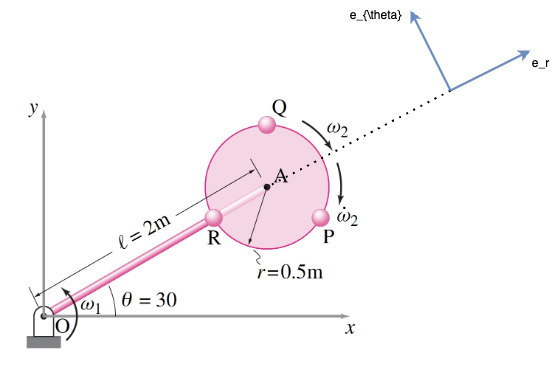
\includegraphics[width=\linewidth]{hw3.png}
    \caption{Annotated Dynamical System}
\end{figure}

\subsection{The velocity of the mass P in the fixed frame xy}

We are asked to $\prescript{O}{}{\vv{v}}^{\, P}$ velocity of mass P relative to the fixed frame and also expressed in the fixed frame defined by unit vectors $\{x, y\}$ where $z$ is normal to the plane. So in order to determine this velocity vector, one must first establish coordinate frames: first is relative to point O in the fixed frame, and the second is relative to point A in the body or corotational frame as shown in the above annotated figure of the dynamical system in this problem.

Since this is a kinematics problem the next thing is to establish positional vectors leveraging the body frame defined above using the configuration of the dynamical system state at this particular snapshot in time. The body frame $e_r$ is aligned along the massless rod which also coincides with the position vector from $R \to A$ and the masses are placed along the disk symmetrically: $120^\circ$ apart from one another. Thus we can see from the body frame that the angles of offset between masses $Q$ and $P$ bisects the $e_r$ axis which implies that the angle between $e_r$ and $e_{\theta}$ is $60^\circ$ and $-60^\circ$ respectively.
\begin{align*}
    & \prescript{O}{}{\vv{r}}^{\, A} = l e_r = 2 e_r \\
    & \prescript{A}{}{\vv{r}}^{\, R} = r e_r = -0.5 e_r \\
    & \prescript{A}{}{\vv{r}}^{\, Q} = r \cos(60^\circ) e_r + r \sin(60^\circ) e_{\theta} = 0.25 e_r + 0.433 e_{\theta} \\
    & \prescript{A}{}{\vv{r}}^{\, P} = r \cos(-60^\circ) e_r - r \sin(-60^\circ) e_{\theta} = 0.25 e_r - 0.433 e_{\theta}
\end{align*}
Next thing is to establish the center of mass of the spinning disk is at point $A$.
\begin{align*}
    & \prescript{A}{}{\vv{r}}_G = \frac{1}{m_R + m_Q + m_P}(m_R \prescript{A}{}{\vv{r}}^{\, R} + m_Q \prescript{A}{}{\vv{r}}^{\, Q} + m_P \prescript{A}{}{\vv{r}}^{\, P}) = \frac{1}{1.5}(\underline{0}) = \underbar{0}
\end{align*}
Since $A$ is at the center of mass of the spinning disk this simplifies the equations of motion to simply be $\prescript{O}{}{\vv{v}}^{\, P} = \prescript{O}{}{\vv{v}}^{\, A} + \prescript{A}{}{\vv{v}}^{\, P}$. Note $w_1$ is a positive angular velocity since it is spinning CCW and since $w_2$ is spinning CW it is negative.
\begin{align*}
    & \prescript{O}{}{\vv{v}}^{\, A} = 2 * \dot{\theta} e_{\theta} = 2 * w_1 e_{\theta} = 6 e_{\theta} \\
    & \prescript{A}{}{\vv{v}}^{\, P} = 0.25 * \dot{\theta} e_{\theta} + 0.433 \dot{\theta} e_r = 0.25 * w_2 e_{\theta} + 0.433 * w_2 e_r = -1.25 e_{\theta} - 2.165 e_r \\
    & \underline{\prescript{O}{}{\vv{v}}^{\, P} = 4.75 e_{\theta} - 2.165 e_r}
\end{align*}
The velocity vector defined above is expressed in the body frame, so we now need to transform the coordinate frame from the body into the fixed frame by the following linear transformation.
\begin{align*}
    & \begin{bmatrix} x \\ y \\ z \end{bmatrix} = \begin{bmatrix} \cos(\theta) & -\sin(\theta) & 0 \\ \sin(\theta) & \cos(\theta) & 0 \\ 0 & 0 & 1 \end{bmatrix} \begin{bmatrix} e_r \\ e_{\theta} \\ z \end{bmatrix}
\end{align*}
Where $\theta = 30^\circ$ so we arrive at the following velocity vector from O to P expressed in the fixed frame.
\begin{align*}
    & \underline{\prescript{O}{}{\vv{v}}^{\, P} = -4.25 x + 3.03 y}
\end{align*}

\subsection{The acceleration of the mass P in the fixed frame xy}

To obtain the acceleration of the mass P relative and expressed in the fixed frame xy we first need to differentiate the velocity vectors relative to the fixed expressed in the body first (or positional vectors twice).
\begin{align*}
    & \prescript{O}{}{\vv{a}}^{\, A} = 2 \ddot{\theta} e_{\theta} - 2 \dot{\theta}^2 e_r = 0 - 2 * w_1^2 e_r = -18 e_r \\
    & \prescript{A}{}{\vv{a}}^{\, P} =  (0.25 \ddot{\theta} + 0.433 \dot{\theta}^2) e_{\theta} + (-0.25 \dot{\theta}^2 + 0.433 \ddot{\theta}) e_r = (0.25 \alpha_2 + 0.433 w_2^2) e_{\theta} + (-0.25 w_2^2 + 0.433 \alpha_2) e_r \\
    & \underline{\prescript{O}{}{\vv{a}}^{\, P} = -22.95e_r + 11.58e_{\theta}}
\end{align*}
The above is the acceleration vector relative to the fixed frame expressed in the body frame, so we need to transform the coordinate frame in the same fashion as part (a).
\begin{align*}
    & \underline{\prescript{O}{}{\vv{a}}^{\, P} = -25.67x - 1.45y}
\end{align*}

\subsection{The linear momentum of the mass P}

The equation of linear momentum is $G = \sum m_i v_i$ however we are solely concerned with the linear momentum of mass P which is simply $G_P = m_P \prescript{O}{}{\vv{v}}^{\, P}$ which is described fully in the fixed inertial frame.
\begin{align*}
    & \underline{G_P = m_P \prescript{O}{}{\vv{v}}^{\, P} = 0.5 * \begin{bmatrix} -4.25x \\ 3.03y \end{bmatrix} = \begin{bmatrix} -2.13x \\ 1.52y \end{bmatrix}}
\end{align*}

\subsection{The net force on the mass P}

The net force is defined as $\sum F_i = \sum m_i a_i$ however like part (c) we are solely concerned with the net force on mass P which is $\sum F_P = m_P \prescript{O}{}{\vv{a}}^{\, P}$ which is described fully in the fixed inertial frame.
\begin{align*}
    & \underline{\sum F_P = m_P \prescript{O}{}{\vv{a}^{\, P}} = 0.5 * \begin{bmatrix} -25.67x \\ -1.45y \end{bmatrix} = \begin{bmatrix} -12.84x \\ -0.72y \end{bmatrix}}
\end{align*}

The above assumes no gravitational force is acting on the masses as the problem doesn't explicitly say whether or not to consider this force. Below is the net force acting on mass P if gravity is considered.
\begin{align*}
    & \underline{\sum F_P = m_P * g y + m_P \prescript{O}{}{\vv{a}^{\, P}} = \begin{bmatrix} -12.84x \\ -5.63y \end{bmatrix}}
\end{align*}

\end{document}